\documentclass{article}

\usepackage{pgf}
\usepackage{tikz}
\usetikzlibrary{arrows, automata}
\begin{document}
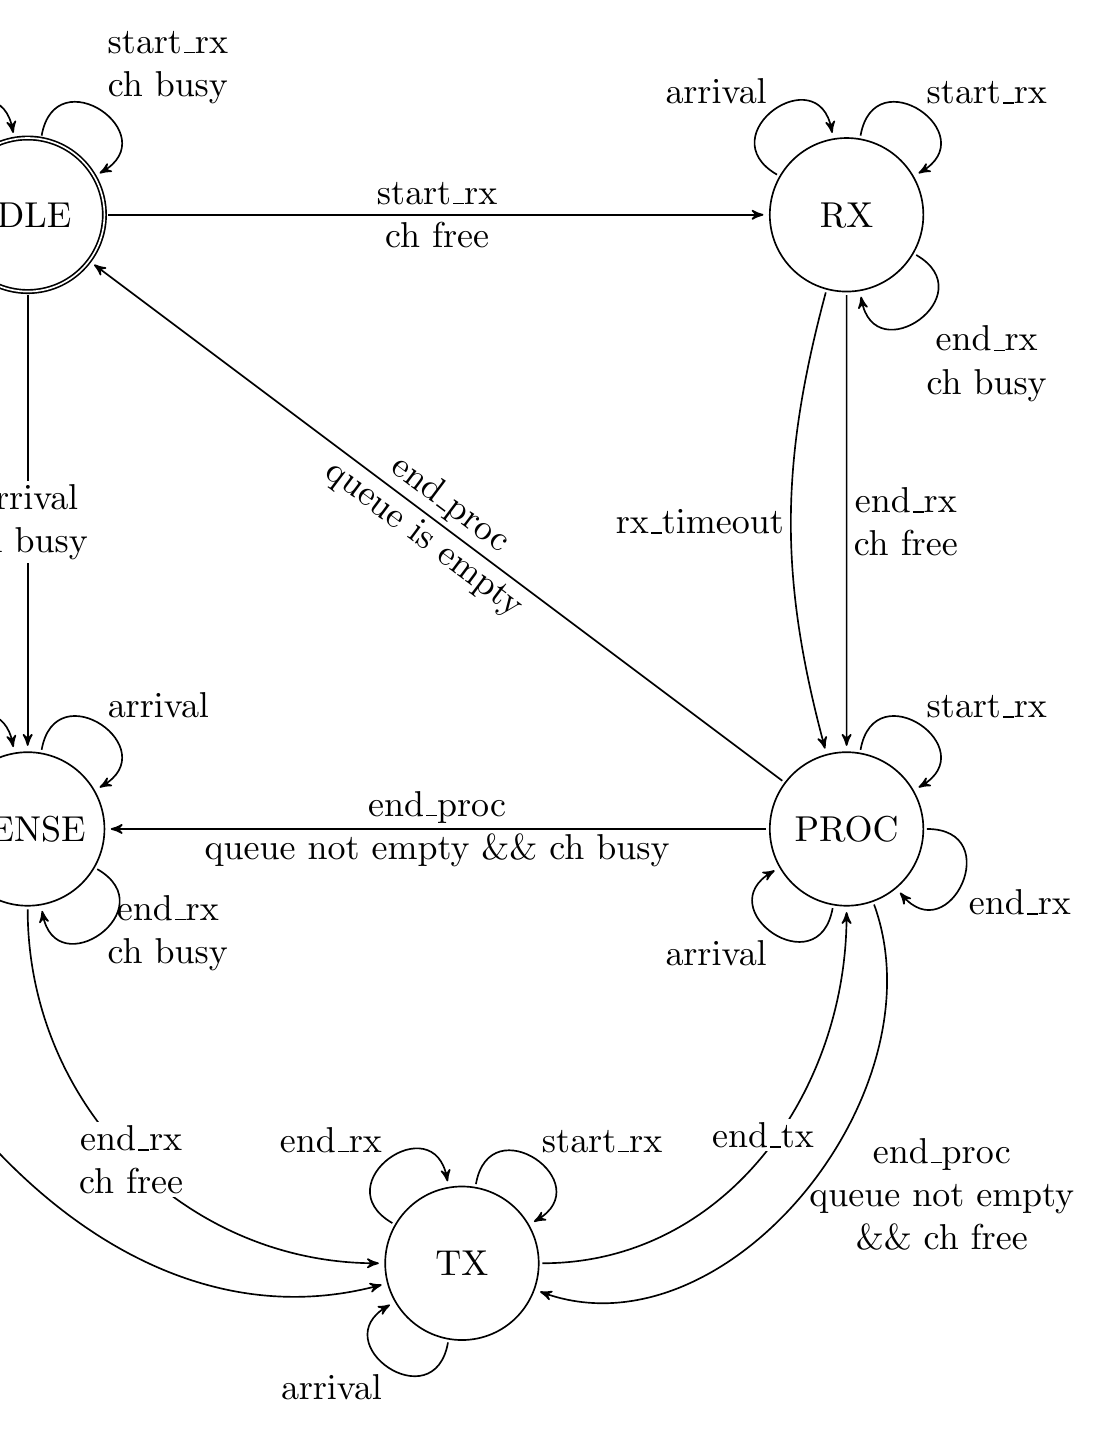
\begin{tikzpicture}[->, >=stealth', shorten >=1pt, auto, node
    distance=6cm, trim left, semithick, outer sep=1pt, inner sep=1pt,
    every node/.style={scale=1.3}, align=center]

  \tikzstyle{every state}=[minimum size=1.5cm]

  \node[state,double] (IDLE) {IDLE};
  \node[state, node distance=8cm] (RX) [right of=IDLE] {RX};
  \node[state]         (SENSE) [below of=IDLE] {SENSE};
  \node[state]         (PROC) [below of=RX] {PROC};
  \node[state]         (TX) [below right of=SENSE] {TX};

  \path[->]
  (IDLE) edge [anchor=center] node {start\_rx\\ch free} (RX)
  edge [anchor=center] node [fill=white] {arrival\\ch busy} (SENSE)
  edge [anchor=center, out=-150, in=-165, looseness=1.1] node
  [fill=white] {arrival\\ch free} (TX)
  edge [out=150,in=100,loop, looseness=3] node {end\_rx} (IDLE)
  edge [out=80,in=30,loop, looseness=3] node {start\_rx\\ch busy} (IDLE)

  (RX) edge node {end\_rx\\ch free} (PROC)
  edge [out=150,in=100,loop, looseness=3] node {arrival} (RX)
  edge [out=80, in=30, loop, looseness=3] node {start\_rx} (RX)
  edge [out=-30, in=-80, loop, looseness=3] node {end\_rx\\ch busy} (RX)
  edge [anchor=east, out=-105, in=105] node {rx\_timeout} (PROC)

  (SENSE) edge [anchor=center, out=-90,in=180] node[fill=white]
  {end\_rx\\ch free} (TX)
  edge [anchor=west, out=-30, in=-80, loop, looseness=3] node
  {end\_rx\\ch busy} (SENSE)
  edge [out=150,in=100,loop, looseness=3] node {start\_rx} (SENSE)
  edge [out=80,in=30,loop, looseness=3] node {arrival} (SENSE)

  (TX) edge [anchor=south, out=0,in=-90] node[fill=white] {end\_tx} (PROC)
  edge [out=-100,in=-150,loop, looseness=3] node {arrival} (TX)
  edge [out=150,in=100, loop, looseness=3] node[fill=white] {end\_rx} (TX)
  edge [out=80,in=30,loop, looseness=3] node {start\_rx} (TX)

  (PROC) edge [sloped, anchor=center] node {end\_proc\\queue is empty} (IDLE)
  edge [anchor=center] node {end\_proc\\queue not empty \&\& ch busy}
  (SENSE)
  edge [anchor=west, out=-70, in=-20, looseness=1] node {end\_proc\\queue not empty\\\&\& ch free} (TX)
  edge [out=80, in=30, loop, looseness=3] node {start\_rx} (PROC)
  edge [out=-00, in=-50, loop, looseness=3] node {end\_rx} (PROC)
  edge [out=-100,in=-150,loop, looseness=3] node {arrival} (PROC);
\end{tikzpicture}
\end{document}
